\section{Heur\'istica Golosa}
\subsection{Explicacion detallada de la heur\'istica propuesta}

La heur\'istica consta de dos etapas: una etapa de inicializaci\'on y luego el algoritmo goloso propiamente dicho.

\subsubsection{Inicializaci\'on}

La etapa de inicializaci\'on consta en calcular los caminos m\'inimos en cuanto a costo $w_1$ de todos los nodos hacia el nodo de llegada. Ya que el grafo es simple, las aristas no tienen orientaci\'on definida, por lo cual dados dos nodos $v_1$ y $v_2$, el camino de $v_1$ a $v_2$ es igual al camino de $v_2$ a $v_1$. Esto nos permite ejecutar una \'unica vez el algoritmo de Dikjstra desde el nodo de llegada hasta todos los dem\'as y obtener lo buscado.

\vspace{2mm}

Una vez obtenidos los caminos m\'inimos de cada nodo a la llegada en cuanto a costo $w_1$, \'estos nos permiten conocer lo siguiente:

\begin{enumerate}
\item Al iniciar el algoritmo, aquellos nodos para las cuales no existe un camino de longitud $w_1 \leq K$ hasta el nodo llegada, los cuales nuestro algoritmo va a ignorar.
\item En medio de la ejecuci\'on del algoritmo, llamando $W_{ac}$ a la acumulac\'on de costos $w_1$ del camino recorrido por el algoritmo hasta ahora, puedo saber si el nodo $x$ de la pro\'oxima arista $(v,x$) a elegir tiene al menos un camino $c$ hasta el nodo llegada tal que, el costo del camino formado por la uni\'on de $c$ y el recorrido hasta ahora es $\leq K$. En caso de no tenerlo, desde ese nodo no hay un camino v\'alido hasta la llegada, por lo tanto nuestro algoritmo va a descartar esta arista y elegir alguna que tenga al menos un camino posible hasta la llegada. Esto lo podemos conocer, ya que la ejecuci\'on de Dijkstra inicial nos brinda el costo $w_1$ del camino m\'inimo desde el nodo $x$ hasta la llegada, por lo tanto  si $W_{ac}$ + $(v,x)$ + $longMinimoCamino(x,llegada)$ $\leq$ $K$ sabemos que existe al menos este camino v\'alido, caso contrario descartamos la arista.
\end{enumerate}


\begin{center}
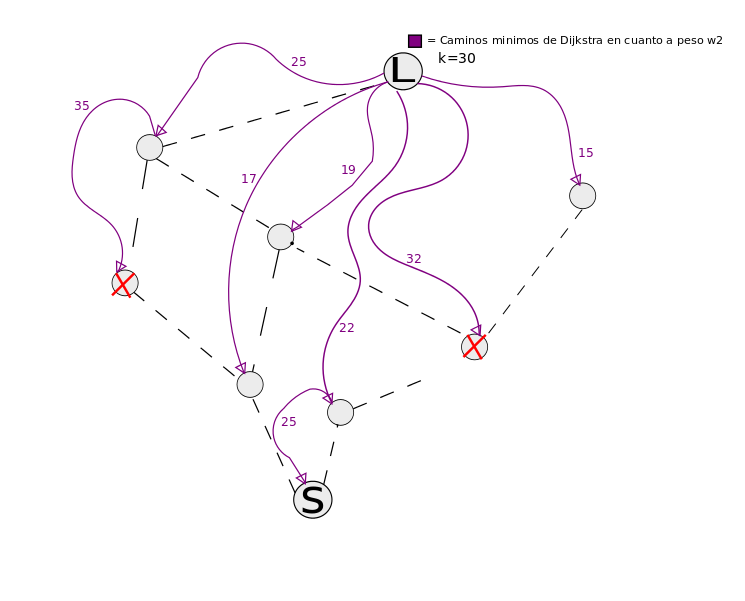
\includegraphics[scale=0.58]{img/inicializacion.png}
\end{center}	
\vspace{2mm}

Este dibujo representa la ejecuci\'on de la inicializaci\'on de la heur\'stica, donde el algoritmo de Dijkstra calcula los costos $w_1$ de los caminos m\'inimos de todos los nodos al nodo llegada (en violeta), y puede verse que aquellos nodos con caminos de costo mayor a $K$ ser\'an descartados.

\vspace{2mm}

Cabe aclarar, que en la implementaci\'on, se ejecuta el algoritmo de Dijkstra ignorando el nodo salida, ya que queremos los caminos m\'inimos desde la llegada hasta todos los nodos sin pasar por el nodo salida, de otra forma no tendr\'a sentido el resultado.

\vspace{2mm}

Esto nos brinda una propiedad invariante: sabemos que en cada iteraci\'on, el costo acumulado del recorrido hecho es menor a $K$, y si al menos existe alg\'un un camino de costo menor a $K$ de salida a destino, el algoritmo muy probablemente va a poder llegar al nodo de llegada (excepto en casos enunciados en la siguiente secci\'on). Deducimos esto al considerar que, o bien no existe ning\'un camino y  el algoritmo termina en la primera iteraci\'on o el algoritmo elige una primera arista (por lo tanto existe un camino). 

\vspace{2mm}

Si el algoritmo elige una primera arista, pero luego no logra llegar a destino, significa (excepto en casos enunciados en la siguiente secci\'on) que en alg\'un punto, desde un nodo $v$ no encontr\'o ninguna arista $(v,x)$ tal que $W_{ac}$ + $(v,x)$ + $longMinimoCamino(x, llegada)$ $\leq$ $K$. Pero esto no puede ocurrir, ya que en la anterior iteraci\'on, tuvo que elegir necesariamente alguna arista con un extremo en $v$, y la elecci\'on de $v$ en la anterior iteraci\'on nos aseguraba que desde $v$ existe alg\'un camino v\'alido hasta la llegada, lo cual es absurdo porque el algoritmo se detuvo cuando lleg\'o a $v$. De esta forma concluimos en que, si existe algu\'n camino v\'alido desde la salida hasta la llegada, entonces nuestro algoritmo en la mayori\'a de los casos va a tener como salida un camino v\'alido (a desarrollar en la secci\'on siguiente).

\subsubsection{Algoritmo goloso}

A continuaci\'on se ejecuta el ciclo principal del algoritmo, que genera el CACM usando una heur\'istica golosa. Luego de la ejecuc\'on inicial del algoritmo de Dijkstra, el ciclo principal comienza en el nodo salida y realiza una elecci\'on golosa, la cual es: desde el nodo $v$, descartar las aristas $(v,x)$ incidentes en $v$ tal que $W_{ac}$ + $ss$ + $longMinimoCamino(x,llegada)$ > $K$. Entre las aristas que quedan, escoger la de menor costo $w_1$.(Aqu\'i se encuentra la desici\'on golosa). El algoritmo itera hasta alcanzar el nodo llegada.

\subsection{Pseudoc\'odigo}

\begin{algorithmic}

\Procedure{$Sol\_Golosa$}{$Grafo\: g, \:vertice\: v_1,\: vertice \: v_2, \: int \: k$}{$\rightarrow lista<eje>\: camino$}

\State $vector<int> \: costos[g.\#nodos]$
\Comment $ O(n) $
\State $ Dijkstra( g, v_2, costos) $
\Comment $ O() $
\State $lista<eje> \: camino= \emptyset$
\Comment $ O(1) $
\State $ int \: costoCamino = 0 $
\Comment $ O(1) $
\State $ vertice \: v_{actual} = v_1 $
\Comment $ O(1) $
\While{ $ actual != v_2 \: || \: incidentes= \emptyset $ }
\Comment $ O(n) $
	\State $ list<eje> \: incidentes = incidentes(v_{actual}, g) $
	\Comment $ O(m) $
	\State $ eje \:	 minimo = cab(incidentes) $
	\Comment $ O(1)$
	\For {each $(u,v) \in \: incidentes$}
	\Comment $ O(m) $
		\If {$ costos(v) + costoCamino \leq k \: \&\& \: costo2(u,v) \leq minimo$}
		\Comment $ O(1) $
			\State $ minimo = (u,v) $
			\Comment $ O(1) $
		\EndIf
	\EndFor
	\State $ Agregar(minimo, camino) $
	\Comment $ O(1) $
	\State $ costoCamino \: += costo1(minimo) $
	\Comment $ O(1) $
	\State $ v_{actual} = v $
	\Comment $ O(1) $
\EndWhile
\State $ return \: camino $
\Comment $ O(1) $

\EndProcedure

\end{algorithmic}


\subsection{Nivel de optimalidad de las soluciones}

A continuaci\'on vamos a exponer casos en los que la heur\'istica es muy poco eficiente.
\subsubsection{Costos $w_1$ despreciables}

La heur\'istica se basa fuertemente en asegurarse de que el costo $w_1$ del camino encontrado efectivamente sea menor a $K$, y por esto, uno de sus principales fuertes es el descarte de aristas para los cuales no existen caminos v\'alidos. Pero, si los costos $w_1$ de las aristas son despreciables, es decir, sus valores son muy pequenos (no nulos), de tal forma que el costo de cualquier camino simple es siempre menor a $K$, el algoritmo entero se reduce a la elecci\'on golosa de, en cada iteraci\'on, elegir la arista incidente de menor peso y agregarla al camino. Esto puede traer consecuencias como \'esta:

\begin{center}
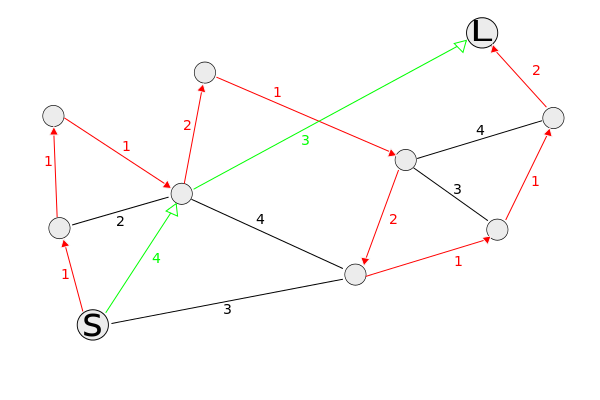
\includegraphics[scale=0.7]{img/grafoCaminoMasLargo.png}
\end{center}
\vspace{2mm}

La familia de grafos en la cual para todo camino simple en el grafo su costo $w_1$ es siempre menor a $k$. En estos casos el m\'etodo de desici\'on y descarte del algoritmo es inefectivo y s\'olo prima la desici\'on golosa. Vemos en este grafo, que el camino formado por la elecci\'on de las aristas de menor coste $w_2$ (en color rojo) desde la salida tiene un coste final $w_2$ m\'as alto que el camino \'optimo (en verde). Los n\'umeros junto a cada arista son los costos $w_2$, y omitimos los costos $w_1$.

\vspace{2mm}

Hay que destacar que podr\'ia generarse un grafo con una suceci\'on arbitrariamente larga de nodos tal que para cada nodo, la arista de menor peso $w_2$ lo lleve al siguiente y evitar de esta forma que el algoritmo encuentre el nodo llegada hasta el final de la suceci\'on. De esta forma, podemos generarnos grafos de esta familia en los cuales la soluci\'on de nuestra heur\'stica est\'a tan lejos de la \'optima como queramos (sin pasarse de la cota $K$).


\begin{center}
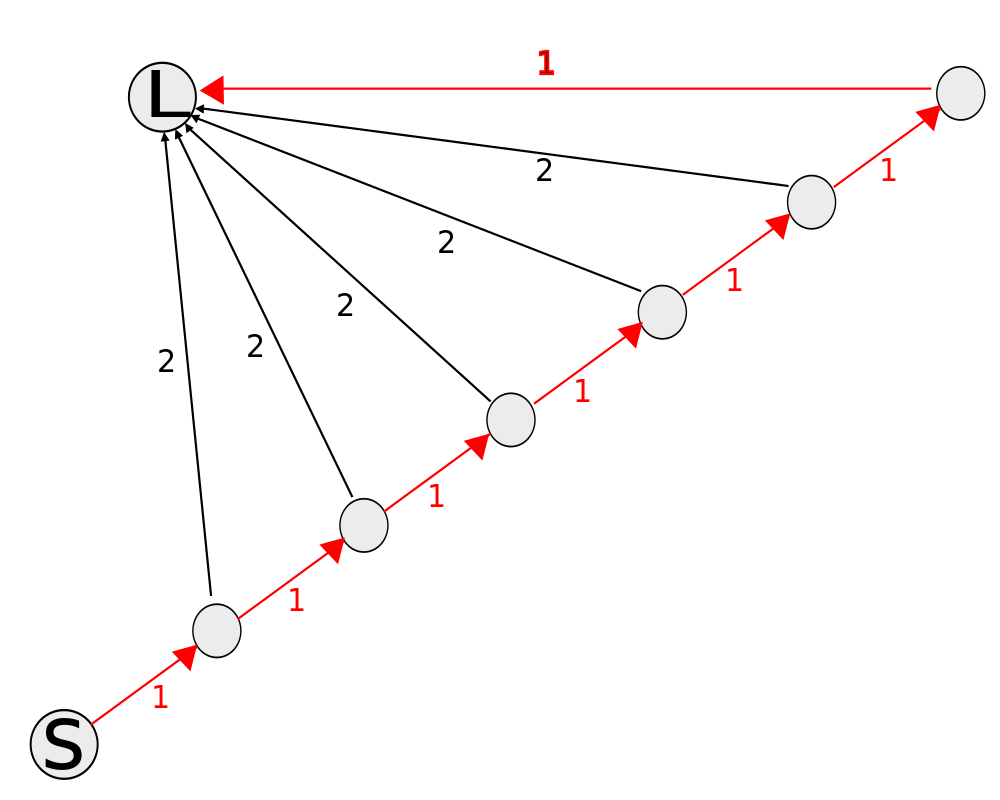
\includegraphics[scale=0.35]{img/grafoChoto.png}
\end{center}

\subsubsection{Costos $w_1$ nulos}

En el caso de que algunas o todas aristas aristas tengan costos $w_1$ nulos, no s\'olo es inefectiva la inicializaci\'on sino que tambi\'en se pierde la certeza de si el algoritmo va a llegar efectivamente a destino, ya que en ning\'un momento hay un impedimento para seguir recorriendo arbitrariamente el grafo (cuando, en el caso en que los costos son no nulos, el hecho de ir acumulando costo $w_1$ necesariamente restring\'ia en alg\'un punto los caminos a tomar a aquellos que llegaban al destino con costo menor a $K$).

\vspace{2mm}

Podemos ver en un ejemplo c\'omo si el grafo posee un conjunto de nodos, tal que sus aristas de menor peso $w_2$ formen un ciclo entre ellos, el algoritmo podr\'a quedarse ciclando infinitamente y no llegar al destino.

\begin{center}
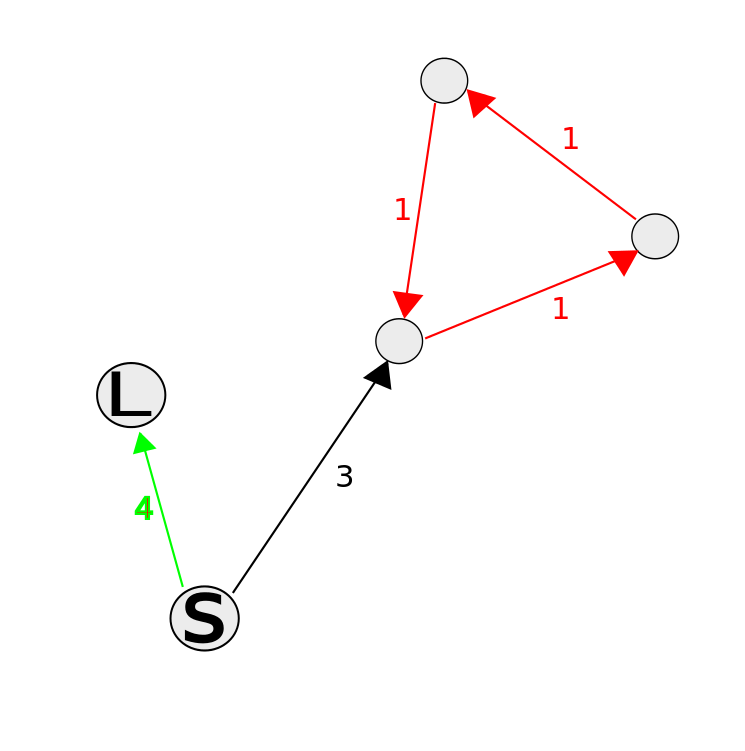
\includegraphics[scale=0.35]{img/ciclo.png}
\end{center}


\section{Heur\'istica Golosa Mejorada}

\subsection{Explicacion detallada de la heur\'istica propuesta}

De forma de solucionar estos problemas y evitar que el algoritmo se aleje arbitrariamente del nodo de llegada , determinamos mejorar la inicializaci\'on de la heur\'istica, y junto con la ejecuc\'on de Dijkstra, realizar una b\'usqueda en anchura BFS, con el objetivo de determinar la distancia en saltos o aristas de todos los nodos a la llegada. De esta forma, si nos aseguramos de que en cada iteraci\'on, la b\'usqueda golosa reduzca esa distancia, el algoritmo va terminar en el nodo destino.

\vspace{2mm}

Esto desencadena en una clara limitaci\'on en los caminos que va a dar como resultado dado que, al pedir que la pr\'oxima arista a elegir reduzca la distancia en saltos a llegada a menos 1 en todas las itereaciones, s\'olo vamos a obtener como resultado caminos con distancia en saltos menor o igual a la distancia en saltos de la salida a la llegada. Pero consideramos que ganamos mucho m\'as con el hecho de asegurarnos que en todo caso el algoritmo termine, llegue al nodo destino, y por medio de un camino v\'alido (si existe al menos uno).

De esta forma, la desici\'on golosa queda:

\begin{enumerate}
\item Entre los nodos para los cuales existe un camino cuyo costo sumado al cumulado es $\leq K$:
\item Entre los nodos que reducen la distancia en saltos a la llegada en al menos 1:
\item Elegir el nodo con la arista de menor peso $w_2$
\end{enumerate}

\subsection{Pseudoc\'odigo}


\begin{algorithmic}

\Procedure{$Sol\_Golosa$}{$Grafo\: g, \:vertice\: v_1,\: vertice \: v_2, \: int \: k$}{$\rightarrow lista<eje>\: camino$}

\State $vector<int> \: costos[g.\#nodos]$
\Comment $ O(n) $
\State $vector<int> \: distancias[g.\#nodos]$
\Comment $ O(n) $
\State $ Dijkstra( g, v_2, costos) $
\Comment $ O() $
\State $ Bfs( g, v_2, distancias) $
\Comment $ O(n+m) $
\State $lista<eje> \: camino= \emptyset$
\Comment $ O(1) $
\State $ int \: costoCamino = 0 $
\Comment $ O(1) $
\State $ int \: distanciaLlegada = distancias[v_1]$
\State $ vertice \: v_{actual} = v_1 $
\Comment $ O(1) $
\While{ $ actual != v_2 \: || \: incidentes= \emptyset $ }
\Comment $ O(n) $
	\State $ list<eje> \: incidentes = incidentes(v_{actual}, g) $
	\Comment $ O(m) $
	\State $ eje \:	 minimo = cab(incidentes) $
	\Comment $ O(1)$
	\For {each $(u,v) \in \: incidentes$}
	\Comment $ O(m) $
		\If {$ costos(v) + costoCamino \leq k \: \&\& \: costo2(u,v) \leq minimo  \&\& distancias(u,v) < distanciaLlegada$}
		\Comment $ O(1) $
			\State $ minimo = (u,v) $
			\Comment $ O(1) $
		\EndIf
	\EndFor
	\State $ Agregar(minimo, camino) $
	\Comment $ O(1) $
	\State $ costoCamino \: += costo1(minimo) $
	\Comment $ O(1) $
	\State $ v_{actual} = v $
	\Comment $ O(1) $
	\State $distanciaLlegada = distanciaLlegada - 1 $
\EndWhile
\State $ return \: camino $
\Comment $ O(1) $

\EndProcedure

\end{algorithmic}

\subsection{Complejidad temporal para el peor caso}

La inicializaci\'on ejecuta el algoritmo de Dijkstra, que tiene una complejidad de $O(n^2)$, y luego un Bfs, $O(n+m)$. El ciclo goloso del algoritmo itera hasta que el v\'ertice actual es igual al v\'ertice de llegada, y va a iterar tantas veces como la distancia en saltos desde el nodo salida hasta el nodo llegada. Est n\'umero est\'a acotado por la cantidad de nodos, por lo que $\in O(n)$. Sabemos que el algoritmo no va a repetir v\'ertices ya que  en cada iteraci\'on se mueve a un nodo con distancia en saltos estrictamente menor al anterior. Al iniciar el ciclo se ejecuta la funci\'on $incidentes$ que recorre las aristas incidentes en el v\'ertice $actual$, como m\'aximo puede haber $m$ aristas por lo tanto tiene complejidad $O(m)$, y se ejecuta un ciclo $for$ que recorre estas aristas incidentes, por lo tanto tambi\'en $\in$ $O(n)$. Esto nos da una complejidad final de = $ O(n^2)+ O(n+m)+ O(n)*(O(m)+O(m)) = O(n^2)$. 

\subsection{Experimentaci\'on de correctitud}

A continuaci\'on aplicamos la heur\'istica a algunos ejemplos de grafos.

\vspace{10mm}

Buscamos el CACM de este grafo del nodo $1$ al nodo $10$, con el l\'mite $K = 5$. Hay 3 caminos posibles. El camino 1 posee un peso $w_1$ total de $4$, y un peso $w_2$ de $10$. El camino 2 posee un peso $w_1$ total de $8$ con lo cual no es un camino v\'alido. El camino 3 tiene un peso $w_1$ total de $5$ y $w_2$ de $10$.


\begin{center}
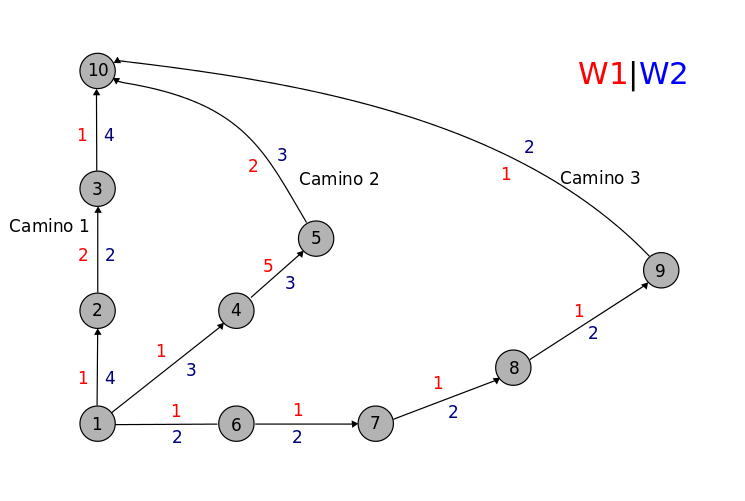
\includegraphics[scale=0.5]{img/grafoGoloso1.png}
\end{center}


Tanto el camino 1 como el camino 3 son soluciones posibles para el algoritmo. El camino 2 deber\'ia ser ignorado. Y dado el c\'odigo que respecta al bfs del algoritmo, deber\'ia descartar el camino 3 ya que moverse al nodo $6$ es alejarse del nodo llegada, ya que el nodo salida se encuentra a distancia $3$ del de llegada y el nodo $6$ se encuentra a distancia $4$.

\vspace{10mm}

Luego de aplicar la heur\'istica a este grafo vemos que efectivamente el algoritmo elige el camino 1.

\vspace{5mm}
Salida del algoritmo:

\begin{lstlisting}[frame=single]
4 10 4 1 2 3 10
\end{lstlisting}

Analicemos los anteriores grafos problem\'aticos.

\begin{center}
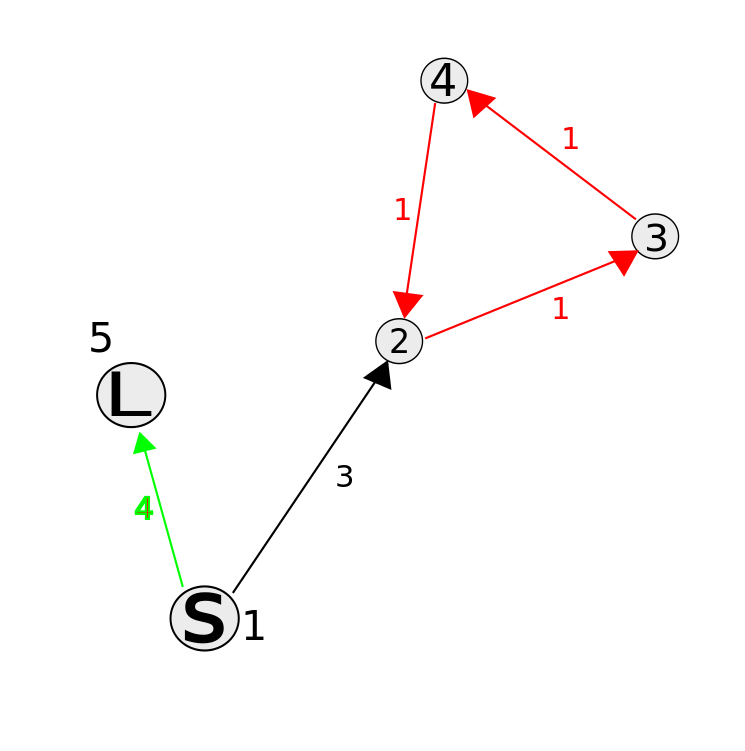
\includegraphics[scale=0.4]{img/cicloNumerado.png}
\end{center}

En este grafo, la heur\'istica sin BFS, al ser los pesos $w_1$ nulos el algoritmo decid\'a tomar la arista m\'as liviana hacia el nodo $2$ y quedaba ciclando. Ahora vemos que la heur\'istica mejorada reconoce que moverse hacia el nodo $2$ es efectivamente alejarse de la llegada y decide tomar la arista hacia la llegada directamente.


\vspace{5mm}
Salida del algoritmo:

\begin{lstlisting}[frame=single]
0 4 2 1 5
\end{lstlisting}

Vemos que de la misma forma la heur\'istica mejorada soluciona el inconveniente de esta familia de grafos, acerc\'andose siempre en 1 en cada paso a la llegada.

\begin{center}
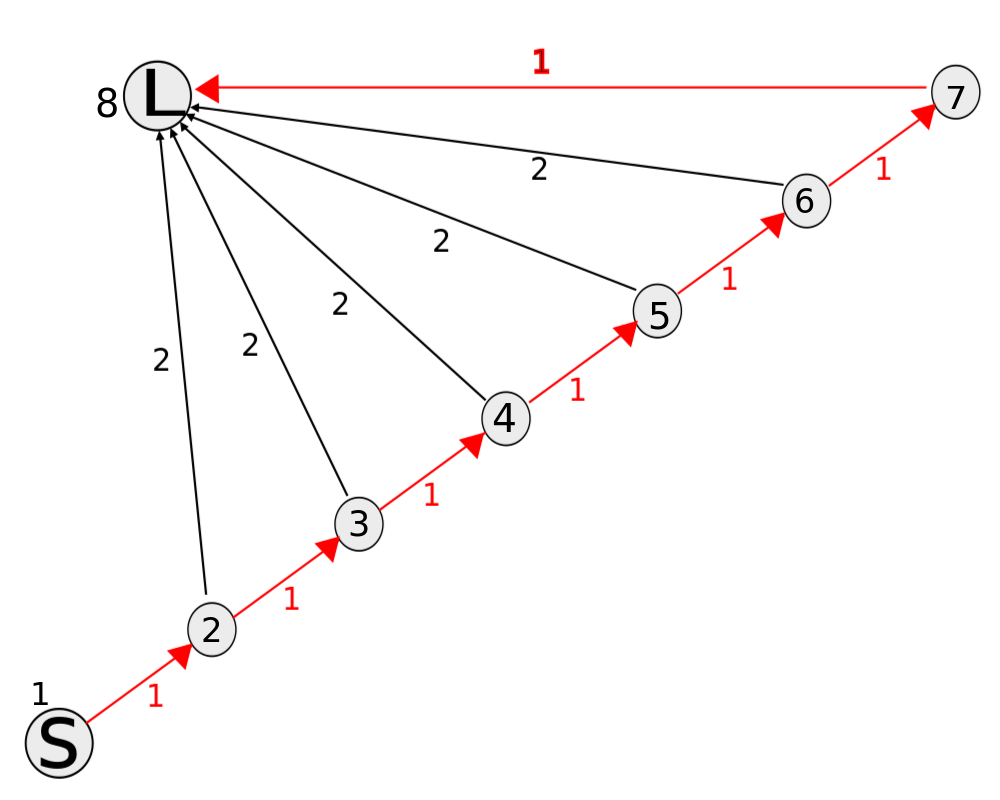
\includegraphics[scale=0.3]{img/grafoChotoNumerado.png}
\end{center}

\vspace{10mm}

Salida del algoritmo:

\begin{lstlisting}[frame=single]
0 3 3 1 2 8
\end{lstlisting}


En el siguiente ejemplo vemos que algunas soluciones siguen siendo sub\'optimas en algunos casos:

\begin{center}
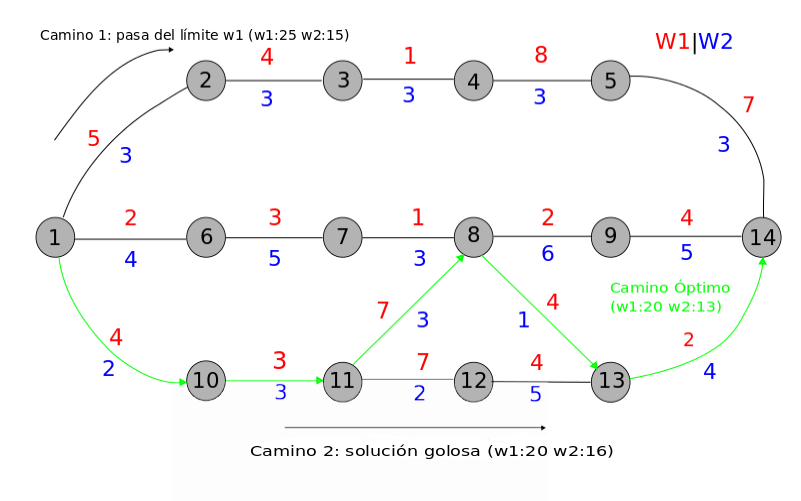
\includegraphics[scale=0.6]{img/grafoMasCompletoGreedy.png}
\end{center}

En este caso en el cual el algoritmo descarta correctamente el camino cuyo peso $w_1$ se pasa de la cota, pero la desici\'on golosa de elegir la arista de menor peso $w_2$ en cada iteraci\'on lo lleva a elegir un camino sub\'optimo. Esto se da generalmente cuando la primera o una de las primeras elecciones lo lleva a tomar un camino que m\'as adelante termina siendo peor, ya que un algoritmo goloso no considera el camino recorrido ni el por recorrer, s\'olo tiene en cuenta las aristas actuales en su desici\'on. Notemos que la soluci\'on del algoritmo goloso no puede alejarse arbitrariamente de la \'optima ya que al menos est\'a acotada por la distancia en saltos del nodo salida a llegada.